\section{Amplificadores operacionales AO}

\subsection{Aspectos básicos}
El AO es un amplificador CC multietapa con una entrada diferencial, es decir, amplifica la diferencia entre las terminales de entrada y no la señal por si sola, conservando la forma de onda.

El AO se representa con el siguiente símbolo:

\begin{figure}[h]
	\centering
	\begin{subfigure}[h]{.45\linewidth}
		\centering
		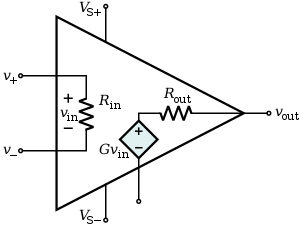
\includegraphics[width = .9\linewidth]{U3_simbolo}
		\caption{Símbolo AO}
		\label{fig:simbolo_AO}
	\end{subfigure}
	\begin{subfigure}[h]{.45\linewidth}
		\centering
		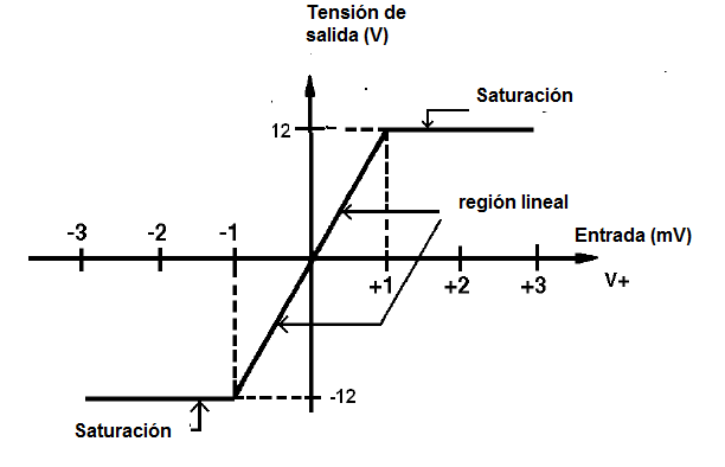
\includegraphics[width = .9\linewidth]{U3_curva}
		\caption{Característica entrada-salida}
		\label{fig:caracteristica}
	\end{subfigure}
	\caption{Amplificador Operacional}
\end{figure}

donde se puden apreciar dos terminales de entrada: la entrada \emph{inversora} (signo negativo) y la entrada \emph{no inversora}. Y una salida. Ademas cuenta con las terminales de alimentación, una positiva $V_{DD}$ y una negativa $V_{EE}$.

La tensión de salida se genera a partir de una fuente de tensión que depende de la diferencia de tensiones en las terminales de entrada multiplicada por un factor A (denominado ganancia):

\begin{equation}
	V_{0} = A (V^{+} - V^{-})
\end{equation}

El signo de la tensión de salida lo determinará a que potencial se encuentra cada entrada.

Esta ecuación se puede ver representada en la figura \ref{fig:caracteristica}  donde se puede apreciar una zona lineal y una zona de saturación, la cual esta determinada por la tensiones de alimentación del AO ($+V_{DD}$ y $-V_{EE}$)

\subsection{Amplificador operacional ideal}
Un amplificador operacional ideal se caracteriza por:

\begin{itemize}
	\item Impedancia de entrada que tiende a infinito.
	\item Impedancia de salida nula.
	\item La salida solo depende de la diferencia entre las tensiones de entrada.
	\item La ganancia diferencial tiende a infinito (ver figura \ref{fig:caracteristica-ideal})
	\item Ancho de banda infinita: el comportamiento no depende de la frecuencia.
\end{itemize}

a\begin{figure}[h]
	\centering
	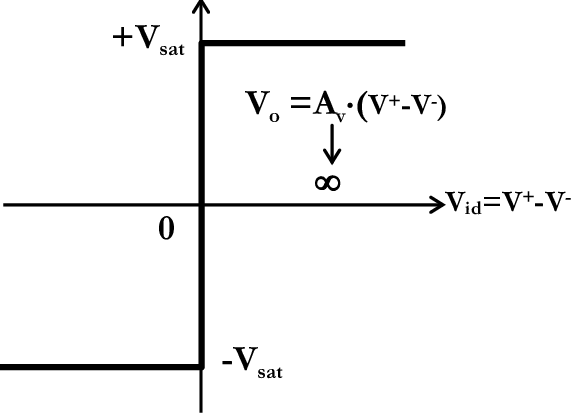
\includegraphics[width= .35\linewidth]{U3_curva_ideal}
	\caption{Amplificador Ideal}
	\label{fig:caracteristica-ideal}
\end{figure}

\subsection{Modos de configuración del AO}

\subsubsection{Sin realimentación}
\subsubsection{Realimentación positiva}
\subsubsection{Realimentación negativa}
